\begin{figure}[htpb!]
%\begin{center}
%\begin{wrapfigure}{r}{5cm}
\rotcaption{Total Recorded Births and Fetal Deaths, 2006-2011}
\label{TEENfig:BirthDeath}
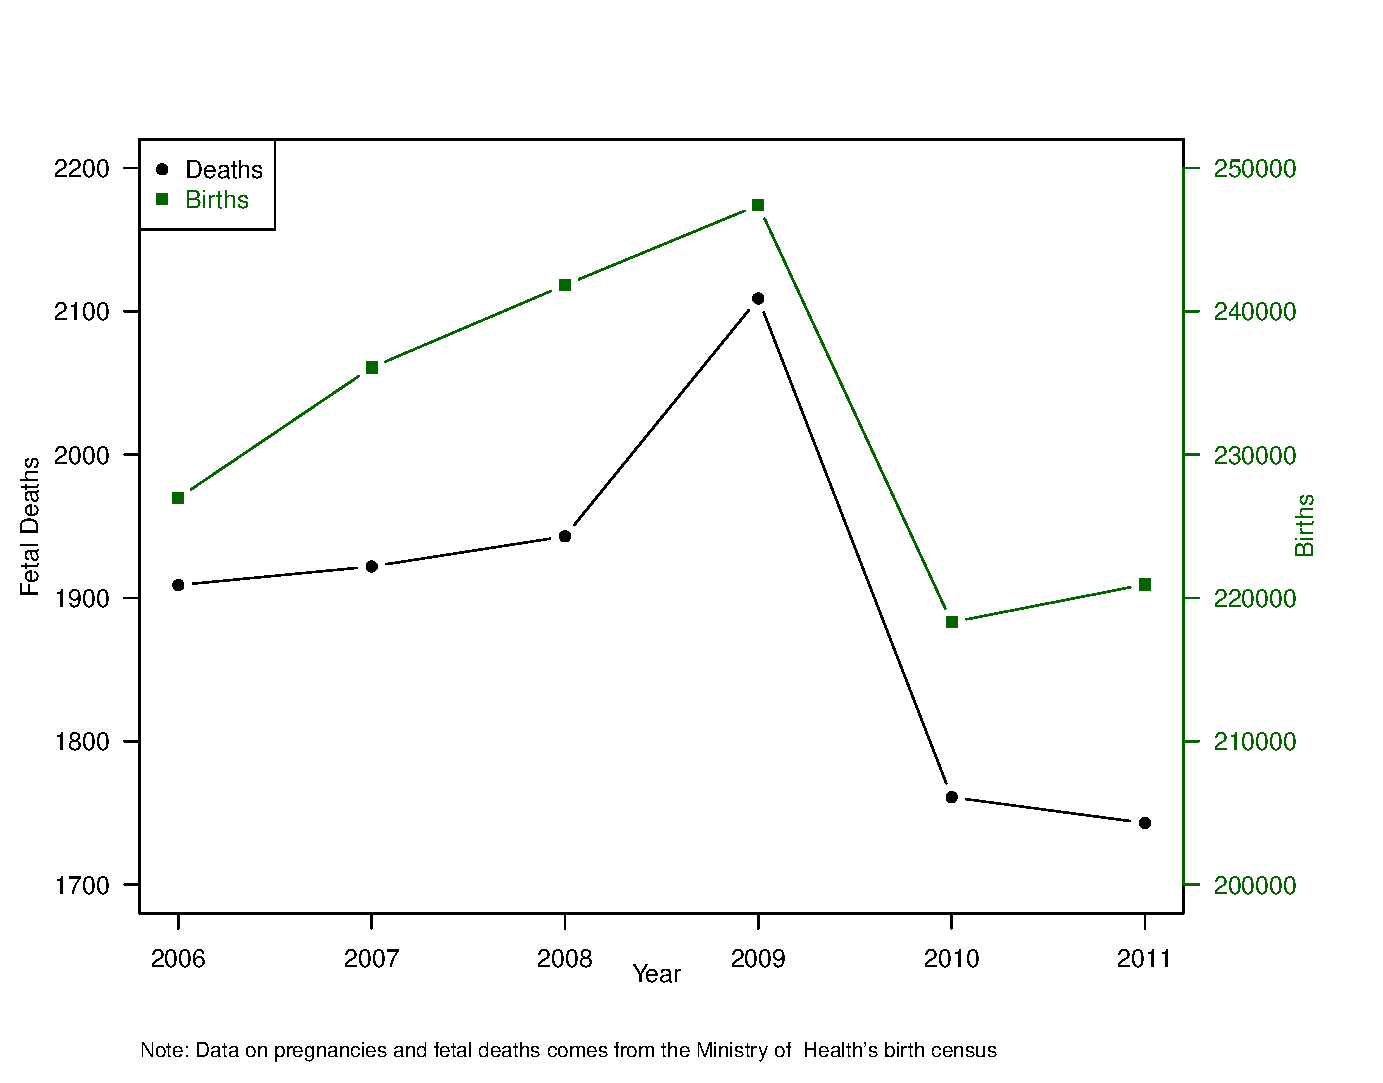
\includegraphics[scale=0.8, angle=90]{\teenfolder/Figures/BirthDeath.eps} 
%\end{center}
\end{figure}

\begin{figure}[htpb!]
\begin{center}
\caption{Pill Prescriptions and Availability by Time}
\vspace{-5mm}
\label{TEENfig:Pilltime}
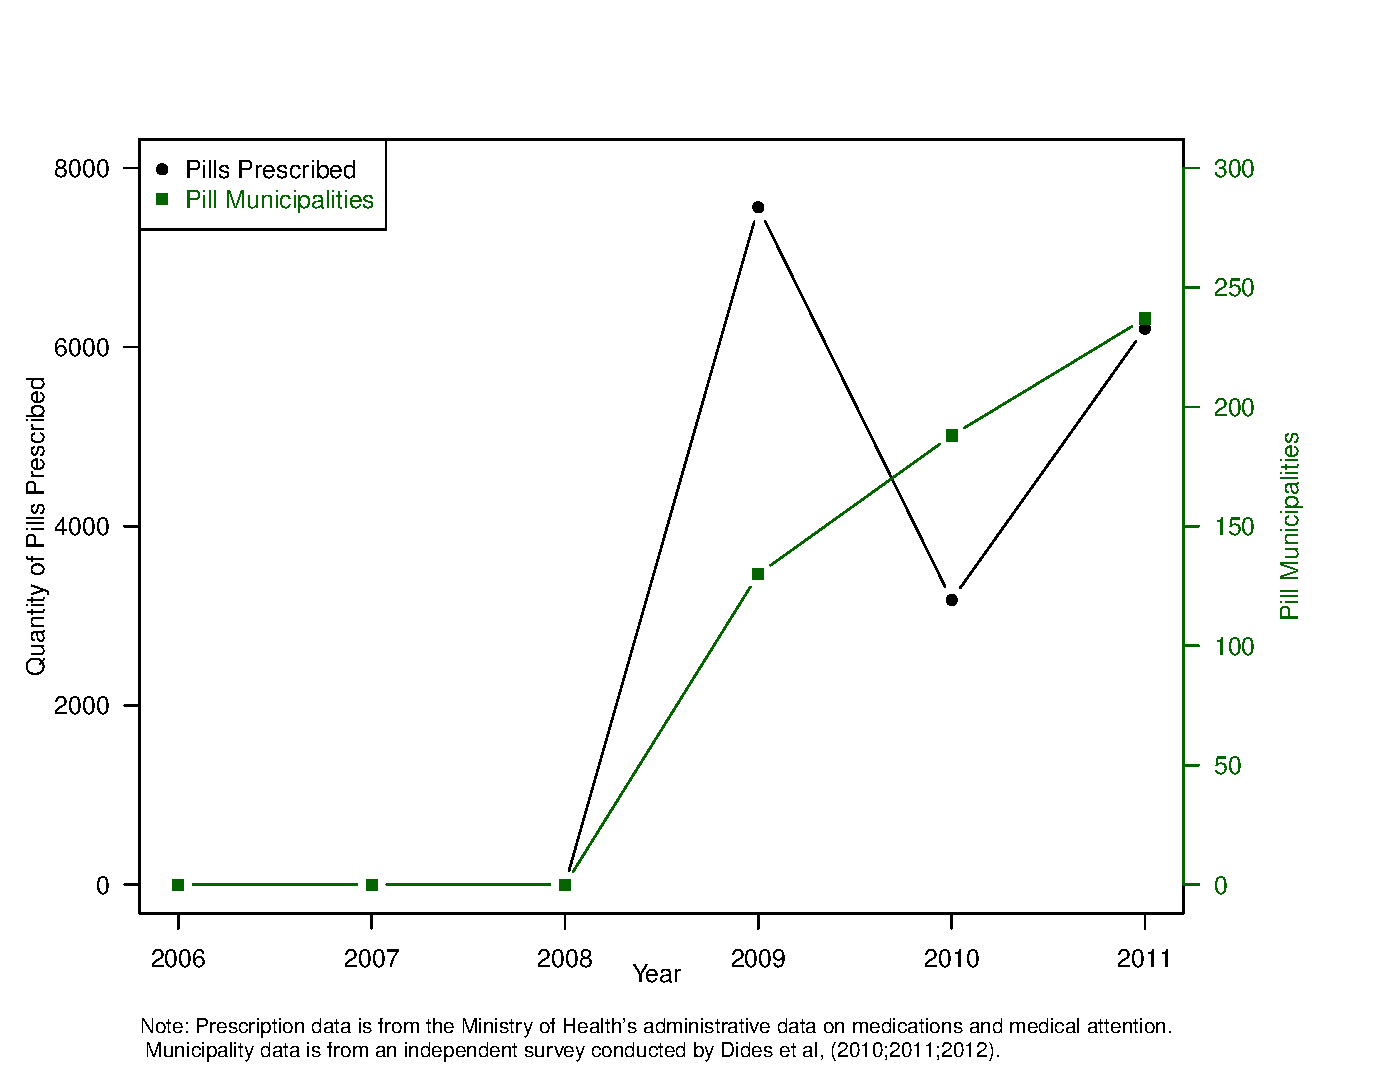
\includegraphics[scale=0.54]{\teenfolder/Figures/Pill.eps} 
\end{center}
\end{figure}

\begin{figure}[htpb!]
\begin{center}
\caption{Pregancies by Age Group and Time}
\vspace{-5mm}
\label{TEENfig:Pregtime}
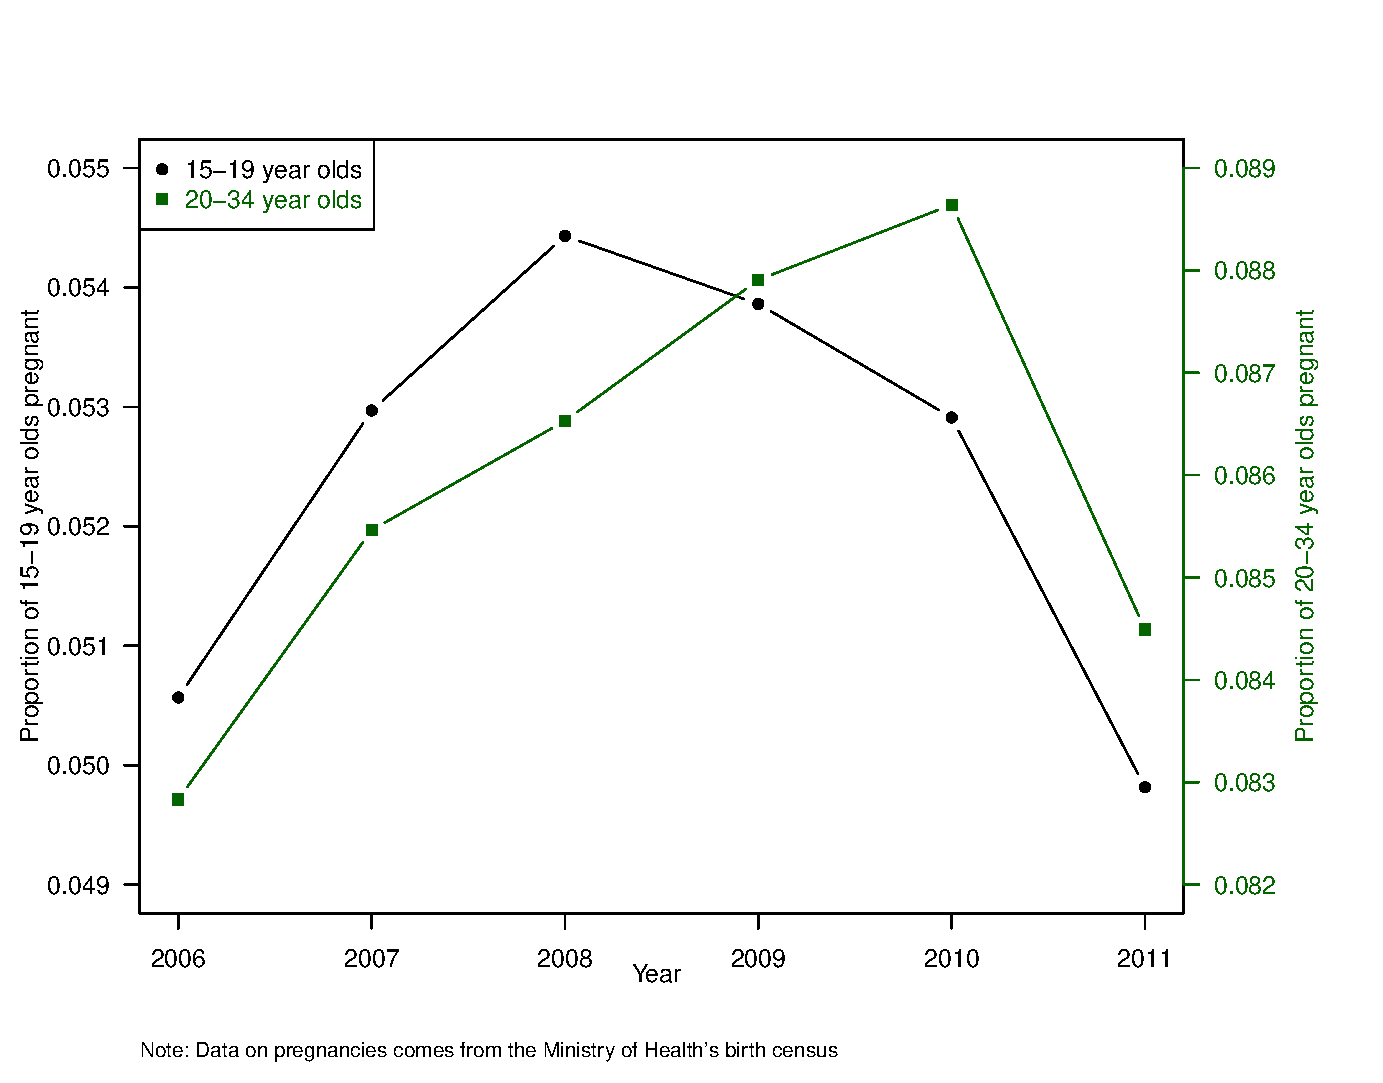
\includegraphics[scale=0.54]{\teenfolder/Figures/Births.eps} 
\end{center}
\end{figure}

\begin{figure}[htpb!]
\begin{center}
\caption{The Availability of the Pill by Geographic Region}
%NOTE: THIS FIGURES HAS BEEN REMOVED TO REDUCE FILE SIZE ON github
\label{TEENfig:PillGeo}
\includegraphics[scale=0.5]{\teenfolder/Results/Pill/Pill_l.eps} 
\end{center}
\end{figure}

\begin{figure}[htpb!]
\begin{center}
\caption{Estimates of $\hat\delta^c$ for Pregnancy (15-19)}
\label{TEENfig:Dist1519}
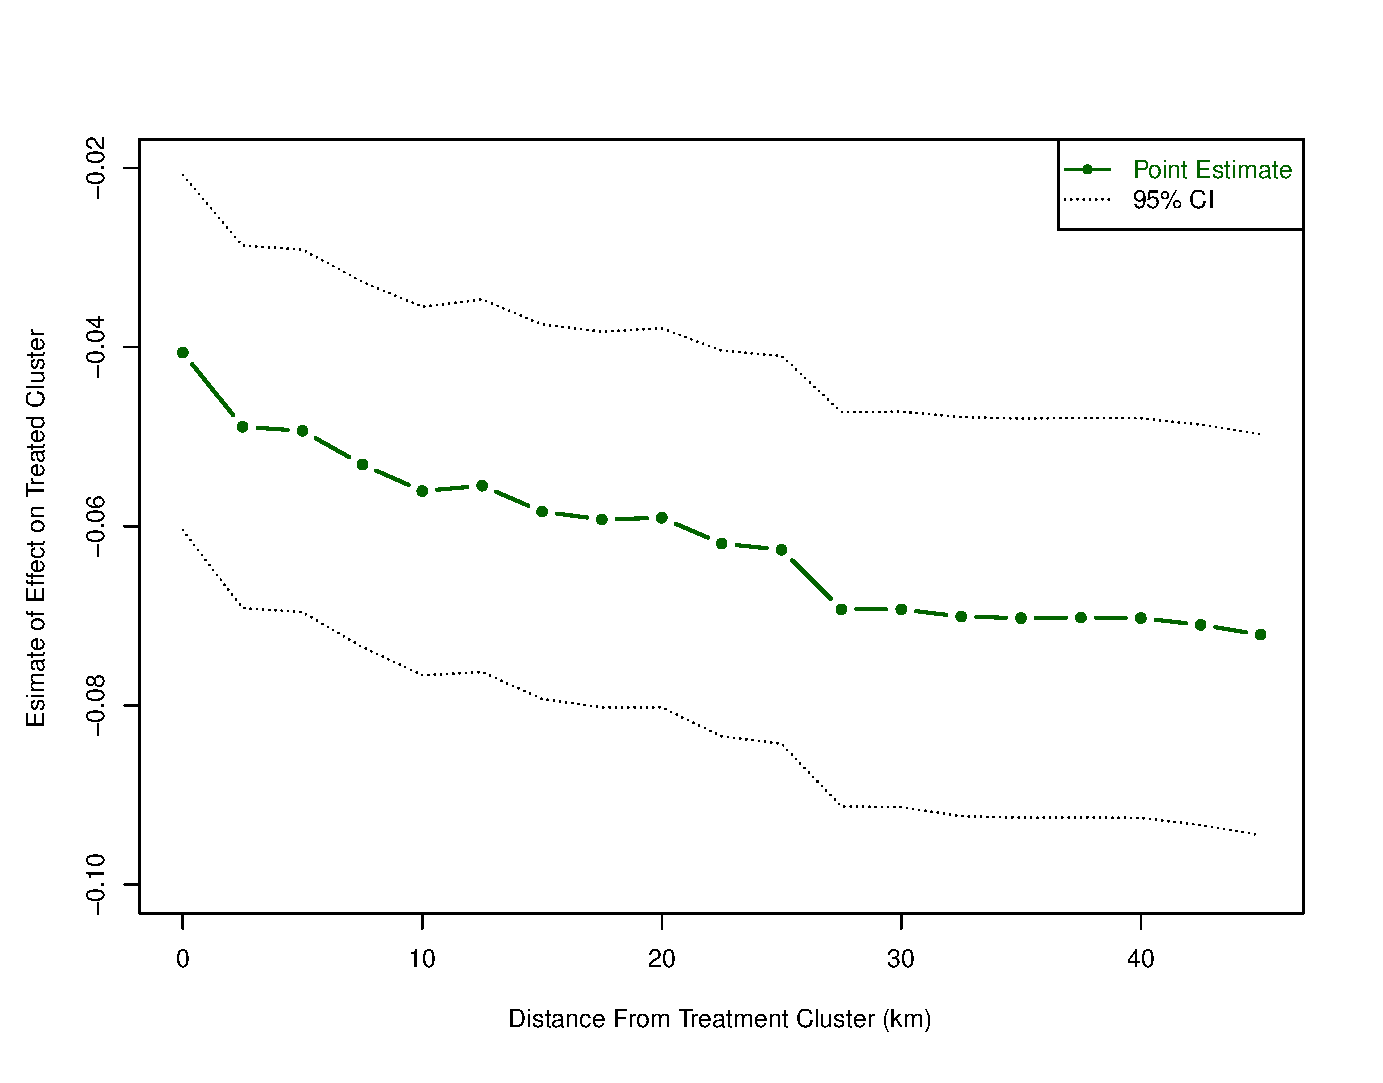
\includegraphics[scale=0.54]{\teenfolder/Figures/Dist1519.eps} 
\end{center}
\end{figure}

\begin{figure}[htpb!]
\begin{center}
\caption{Estimates of $\hat\delta^c$ for Pregnancy (20-34)}
\label{TEENfig:Dist2034}
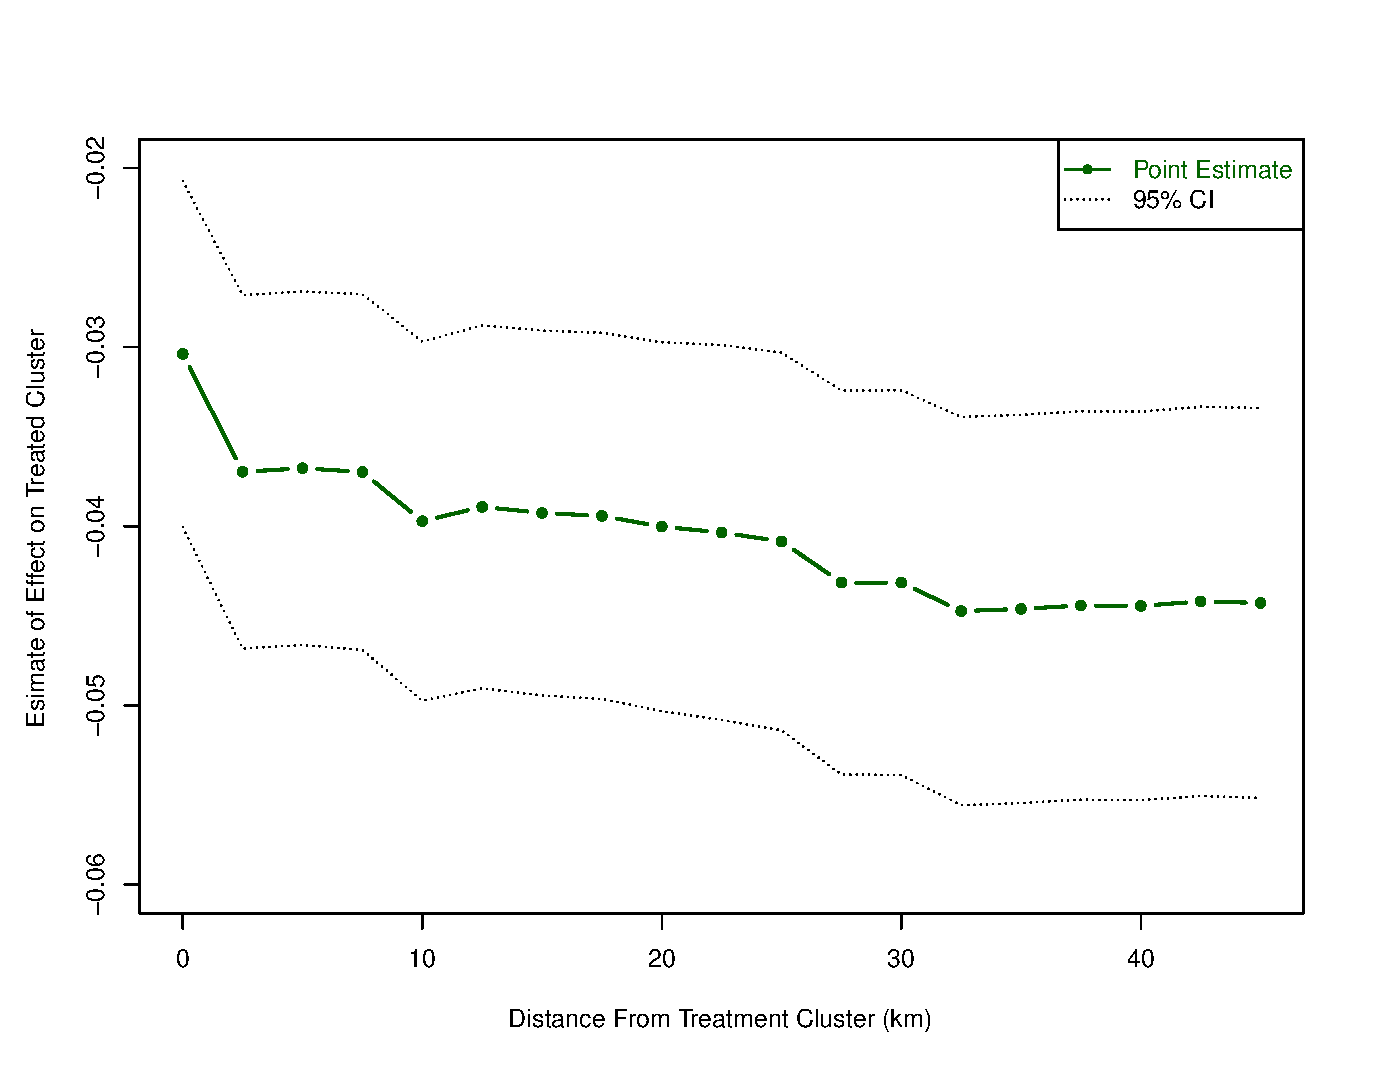
\includegraphics[scale=0.54]{\teenfolder/Figures/Dist2034.eps} 
\end{center}
\end{figure}

\begin{figure}[htpb!]
\begin{center}
\caption{Event Study: 15-19 Years}
\vspace{-5mm}
\label{TEENfig:Event1519}
\includegraphics[scale=0.54]{\teenfolder/Figures/Event1519.eps} 
\end{center}
\end{figure}

\begin{figure}[htpb!]
\begin{center}
\caption{Event Study: 20-34 Years}
\vspace{-5mm}
\label{TEENfig:Event2034}
\includegraphics[scale=0.54]{\teenfolder/Figures/Event2034.eps} 
\end{center}
\floatfoot{Note to figures \ref{TEENfig:Event1519}-\ref{TEENfig:Event2034}:
Points and confidence intervals represent estimates for a full event study.
Each point represents an indicator for the treatment group (pill municipality) 
interacted with $n$ years
prior or posterior to the reform.  On the $x$-axis, 0 represents the first year the 
reform arrived, 1 represents the reform having run for one year, and so forth.  
The (arbitrarily chosen) omitted base in each case is 3 years prior to the reform.}
\end{figure}
